\documentclass[
11pt, % The default document font size, options: 10pt, 11pt, 12pt
codirector, % Uncomment to add a codirector to the title page
]{charter} 




% El títulos de la memoria, se usa en la carátula y se puede usar el cualquier lugar del documento con el comando \ttitle
\titulo{Robot de exploración ambiental} 

% Nombre del posgrado, se usa en la carátula y se puede usar el cualquier lugar del documento con el comando \degreename
\posgrado{Carrera de Especialización en Sistemas Embebidos} 
%\posgrado{Carrera de Especialización en Internet de las Cosas} 
%\posgrado{Carrera de Especialización en Intelegencia Artificial}
%\posgrado{Maestría en Sistemas Embebidos} 
%\posgrado{Maestría en Internet de las cosas}

% Tu nombre, se puede usar el cualquier lugar del documento con el comando \authorname
\autor{Ing. Gonzalo F. Carreño} 

% El nombre del director y co-director, se puede usar el cualquier lugar del documento con el comando \supname y \cosupname y \pertesupname y \pertecosupname
\director{Ing. Sergio Alberino}
\pertenenciaDirector{FIUBA} 
% FIXME:NO IMPLEMENTADO EL CODIRECTOR ni su pertenencia
\codirector{CODIRECTOR} % para que aparezca en la portada se debe descomentar la opción codirector en el documentclass
\pertenenciaCoDirector{FIUBA}

% Nombre del cliente, quien va a aprobar los resultados del proyecto, se puede usar con el comando \clientename y \empclientename
\cliente{Lic. Mariano Landini}
\empresaCliente{-}

% Nombre y pertenencia de los jurados, se pueden usar el cualquier lugar del documento con el comando \jurunoname, \jurdosname y \jurtresname y \perteunoname, \pertedosname y \pertetresname.
\juradoUno{Nombre y Apellido (1)}
\pertenenciaJurUno{pertenencia (1)} 
\juradoDos{Nombre y Apellido (2)}
\pertenenciaJurDos{pertenencia (2)}
\juradoTres{Nombre y Apellido (3)}
\pertenenciaJurTres{pertenencia (3)}
 
\fechaINICIO{13 de marzo de 2023}		%Fecha de inicio de la cursada de GdP \fechaInicioName
\fechaFINALPlan{18 de mayo de 2023} 	%Fecha de final de cursada de GdP
\fechaFINALTrabajo{20 de noviembre de 2023}	%Fecha de defensa pública del trabajo final


\begin{document}

\maketitle
\thispagestyle{empty}
\pagebreak


\thispagestyle{empty}
{\setlength{\parskip}{0pt}
\tableofcontents{}
}
\pagebreak


\section*{Registros de cambios}
\label{sec:registro}


\begin{table}[ht]
\label{tab:registro}
\centering
\begin{tabularx}{\linewidth}{@{}|c|X|c|@{}}
\hline
\rowcolor[HTML]{C0C0C0} 
Revisión & \multicolumn{1}{c|}{\cellcolor[HTML]{C0C0C0}Detalles de los cambios realizados} & Fecha      \\ \hline
0      & Creación del documento.                                 &\fechaInicioName \\ \hline
1      & Se completa hasta el punto 5 inclusive.                 & 14 de marzo de 2023 \\ \hline
2      & Se completa hasta el punto 9 inclusive	y se agregan correcciones.				& 21 de marzo de 2023 \\ \hline
3      & Se completa hasta el punto 12 inclusive y se agregan correcciones. 				& 29 de marzo de 2023 \\ \hline
%		  Se puede agregar algo más \newline
%		  En distintas líneas \newline
%		  Así                                                    & dd/mm/aaaa \\ \hline
%3      & Se completa hasta el punto 11 inclusive                & dd/mm/aaaa \\ \hline
%4      & Se completa el plan	                                 & dd/mm/aaaa \\ \hline
\end{tabularx}
\end{table}

\pagebreak



\section*{Acta de constitución del proyecto}
\label{sec:acta}

\begin{flushright}
Buenos Aires, \fechaInicioName
\end{flushright}

\vspace{2cm}

Por medio de la presente se acuerda con el \authorname\hspace{1px} que su Trabajo Final de la \degreename\hspace{1px} se titulará ``\ttitle'', consistirá esencialmente en \textcolor{black}{la implementación de un prototipo de un sistema embebido para un dispositivo móvil controlado a distancia con funcionalidades que permiten explorar el entorno}, y tendrá un presupuesto preliminar estimado de \textcolor{red}{760} h de trabajo y \textcolor{red}{\$14.000}, con fecha de inicio \fechaInicioName\hspace{1px} y fecha de presentación pública \fechaFinalName.

Se adjunta a esta acta la planificación inicial.

\vfill

% Esta parte se construye sola con la información que hayan cargado en el preámbulo del documento y no debe modificarla
\begin{table}[ht]
\centering
\begin{tabular}{ccc}
\begin{tabular}[c]{@{}c@{}}Dr. Ing. Ariel Lutenberg \\ Director posgrado FIUBA\end{tabular} & \hspace{2cm} & \begin{tabular}[c]{@{}c@{}}\clientename \\ \empclientename \end{tabular} \vspace{2.5cm} \\ 
\multicolumn{3}{c}{\begin{tabular}[c]{@{}c@{}} \supname \\ Director del Trabajo Final\end{tabular}} \vspace{2.5cm} \\
%\begin{tabular}[c]{@{}c@{}}\jurunoname \\ Jurado del Trabajo Final\end{tabular}     &  & \begin{tabular}[c]{@{}c@{}}\jurdosname\\ Jurado del Trabajo Final\end{tabular}  \vspace{2.5cm}  \\
%\multicolumn{3}{c}{\begin{tabular}[c]{@{}c@{}} \jurtresname\\ Jurado del Trabajo Final\end{tabular}} \vspace{.5cm}                                                                     
\end{tabular}
\end{table}




\section{1. Descripción técnica-conceptual del proyecto a realizar}
\label{sec:descripcion}

\begin{consigna}{black} % El bloque "consigna" se usa para poner texto en rojo y dar una pequeña ayuda sobre cómo completar la sección. En cada entrega parcial deben eliminar los comandos begin y end del bloque consigna de las secciones que hayan completado.
El presente proyecto es un emprendimiento personal que busca volcar los conocimientos aprendidos de diseño y programación de sistemas embebidos tomando como caso de uso un robot de exploración ambiental. 

En una primera versión el dispositivo tendrá las funciones básicas de poder desplazarse, sensar el medio ambiente, ser controlado por un mando a distancia de manera cableada y comunicar las diferentes mediciones al control de mandos para su visualización.


\textit{\textbf{Estado del arte:}}
los robots exploradores son dispositivos robotizados que han sido creados con el fin de reconocer y explorar un lugar o terreno siendo capaces de moverse de forma autónoma o controlados por personas a control remoto. Su objetivo es evitar poner en riesgo la vida de los humanos, ya sea debido a que el lugar es inaccesible o porque se encuentra en una zona contaminada.
Tienen como finalidad hacer reconocimiento allí en donde el hombre no puede llegar por ser una zona inaccesible o porque supondría un peligro para la salud. También son utilizados en lugares de difícil acceso, a donde sí que podría llegar una persona solo que empleando más tiempo y recursos económicos.
Una de sus principales características es que están diseñados para moverse por terrenos con alta dificultad para desplazarse. En función de las necesidades del entorno en el que van a trabajar, disponen de diferentes sistemas de motricidad, como son los bípedos o cuadrúpedos, a los que hay sumar los que se mueven por medio de una oruga.
En cuanto a la forma de control, se pueden manejar por control remoto, habiendo equipos más sofisticados que gracias a aplicaciones controladas por Inteligencia Artificial están preparados para desplazarse y tomar decisiones de forma autónoma.
Algunos de los tipos de robots exploradores más conocidos son: robots exploradores espaciales, robots exploradores de minas, robots exploradores de rescate en catástrofes, robots exploradores de tuberías, robots exploradores acuáticos y/o submarinos, etc.

En el siguiente diagrama se puede apreciar el diseño a alto nivel del sistema embebido del robot.

\begin{figure}[htpb]
\centering 
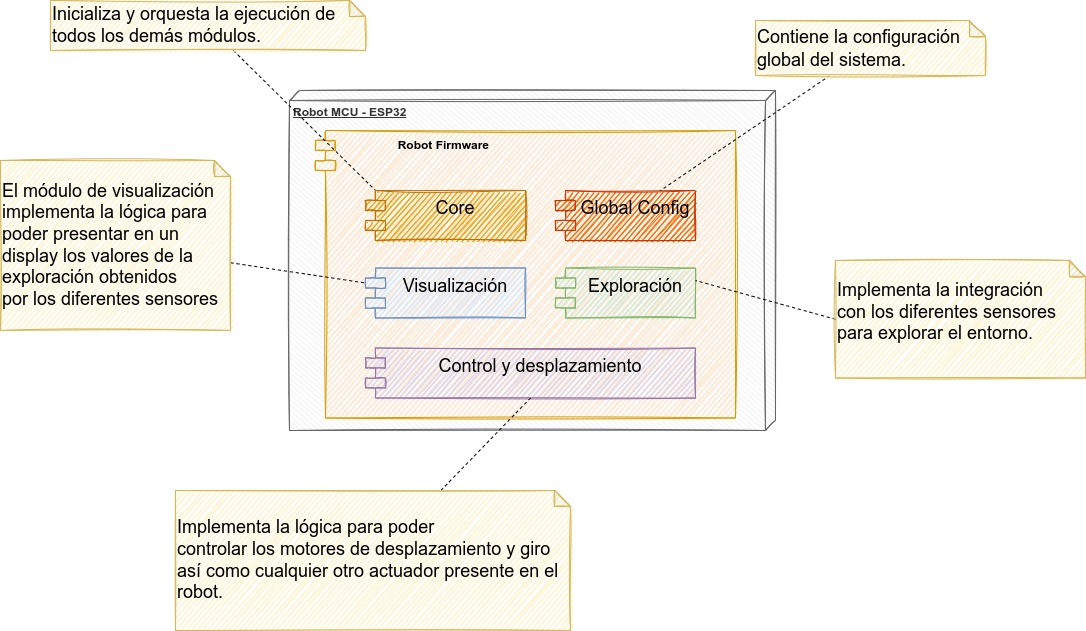
\includegraphics[width=.9\textwidth]{./Figuras/ProyectoFinal-Page-7.jpg}
\caption{Diagrama en bloques del sistema.}
\label{fig:diagBloques}
\end{figure}

\vspace{25px}


\end{consigna}

\section{2. Identificación y análisis de los interesados}
\label{sec:interesados}
\begin{consigna}{black} % este comando se debe borrar para la entrega, junto con la contraparte \end{consigna}{red} 
A continuación se enumeran los diferentes roles e individuos que participarán en el proyecto.
\begin{table}[ht]
%\caption{Identificación de los interesados}
%\label{tab:interesados}
\begin{tabularx}{\linewidth}{@{}|l|X|X|l|@{}}
\hline
\rowcolor[HTML]{C0C0C0} 
Rol           & Nombre y Apellido & Organización 	& Puesto 	\\ \hline

Cliente       & \clientename      &\empclientename	&  -      	\\ \hline
Responsable   & \authorname       & FIUBA        	& Alumno 	\\ \hline
Orientador    & \supname	      & \pertesupname 	& Director Trabajo final \\ \hline
\end{tabularx}
\end{table}


\end{consigna} % este comando se debe borrar para la entrega, junto con la contraparte \begin{consigna}{red}



\section{3. Propósito del proyecto}
\label{sec:proposito}

\begin{consigna}{black}
El propósito de este proyecto es volcar en un caso de la industria los conocimientos más importantes aprendidos en la especialización de sistemas embebidos.

Finalmente, cabe destacar, que si bien el robot de exploración ambiental del presente proyecto es una implementación abstracta con a funcionalidades genéricas (detalladas más adelante en la sección Alcance del Proyecto), su arquitectura podría ser extrapolada a casos de uso más interesantes y de valor en la industria como por ejemplo la exploración de suelos en el agro, la exploración submarina para la perforación de pozos de petróleo, o los antes mencionados en el estado del arte.

\end{consigna}

\section{4. Alcance del proyecto}
\label{sec:alcance}

\begin{consigna}{black}
Las funcionalidades incluidas en el alcance del proyecto serán:
\begin{itemize}
	\item Sistema de desplazamiento terrestre.
	\item Operaciones de exploración (como por ejemplo medición de humedad, temperatura, presión ambiental, etc).
	\item Visualización de estado de exploración (lecturas de los sensores).
	\item Sistema de control por medio de un Joystick cableado.
\end{itemize}

Queda fuera del alcance:
\begin{itemize}
	\item locomoción por cualquier otro medio que no sea terrestre,
	\item cualquier otra función no contemplada en este alcance.
\end{itemize}
\end{consigna}


\section{5. Supuestos del proyecto}
\label{sec:supuestos}

\begin{consigna}{black}
Para el desarrollo del presente proyecto se supone que: 

\begin{itemize}
	\item será posible conseguir los componentes materiales necesarios,
	\item se dispondrá del conjunto de librerías, drivers y APIs de bajo nivel para el desarrollo de las funcionalidades planteadas en el alcance sin ser necesario el desarrollo de drivers y dichos componentes de bajo nivel,
	\item los componentes open source de la comunidad de software libre utilizados a bajo nivel para el acceso al hardware de sensores y actuadores se encontrará estable para que su integración en el proyecto no resulte en desvíos,	
	\item tanto el prototipado de los componentes de software del sistema embebido como el ensamblado de los componentes de hardware del dispositivo no producirán desvíos considerables en el plan,
	\item no habrá desvíos no contemplados en el plan que impidan o demoren entregas en el proyecto,
	\item el comité académico encargado de la corrección tendrá disponibilidad para realizar la evaluación en las fechas planificadas de entrega,
	\item el director asignado tendrá la disponibilidad de tiempo para darle seguimiento al proyecto.
	\item el alumno contará con una disponibilidad de 5 horas diarias (incluyendo fines de semana) para el desarrollo del proyecto en el tiempo convenido.
\end{itemize}


\end{consigna}

\section{6. Requerimientos}
\label{sec:requerimientos}
\begin{consigna}{black}
A continuación se listan los requerimientos del producto:
\begin{enumerate}	
	\item Requerimientos funcionales		
	\begin{enumerate}			
		\item El sistema debe contar con funciones de desplazamiento para poder moverse hacia adelante y atrás, y poder girar radialmente hasta un ángulo de 360 grados.			
		\item El sistema debe ser capaz de realizar las siguientes operaciones de exploración:			
			\begin{enumerate}				
				\item medición de humedad en el ambiente,				
				\item medición de temperatura en el ambiente,				
				\item medición de luminosidad en el ambiente,				
				\item medición de presión ambiental.			
			\end{enumerate}			
		\item El sistema debe poder ser controlado a distancia mediante un joystick para que el dispositivo pueda realizar sus movimientos. En caso de que alguna de sus operaciones de exploración requiera algún mecanismo de control, el mismo también será integrado en el joystick.		
		\item El sistema debe proveer un mecanismo de visualización de las operaciones de exploración al usuario que controla el dispositivo para poder ver el estado y lectura de las operaciones de exploración.		
		\end{enumerate}	
	\item Requerimientos de documentación		
		\begin{enumerate}			
			\item Documentación de arquitectura técnica a alto nivel del diseño del sistema.			
			\item Documentación técnica de la implementación del software.			
			\item Documentación técnica de la implementación del hardware.			
			\item Manual de usuario.	
			\item Informe de avance.
			\item Memoria final.	
		\end{enumerate}	
	\item Requerimiento de testing		
		\begin{enumerate}			
			\item Se debe incluir tests de integración de componentes.		
		\end{enumerate}	
	\item Requerimientos de la interfaz		
		\begin{enumerate}			
			\item La interfaz de usuario debe permitir visualizar las lecturas de cada uno de los sensores.			
			\item Debe haber una pequeña leyenda de la magnitud que se está midiendo y la unidad utilizada junto con el valor.		
		\end{enumerate}	
	\item Requerimientos opcionales		
		\begin{enumerate}			
			\item De interfaz: se permite agregar cualquier otra interfaz adicional que agregue mejoras en la experiencia de usuario			
			\item De operaciones de exploración: se permite agregar cualquier otra operación adicional de exploración que agregue valor a exploración.	
			\item De comunicación: se permite agregar comunicación inalámbrica.		
	\end{enumerate}
\end{enumerate}




\end{consigna}

\section{7. Historias de usuarios (\textit{Product backlog})}
\label{sec:backlog}

\begin{consigna}{black}
A continuacion se listan las historias de usuario. La ponderacion de \textit{story points} se realiza considerando 1 punto = 1 hora:
\begin{itemize}
	\item (150 puntos) Como explorador quiero ver las lecturas de exploración en un display, indicando las magnitudes y unidades usadas para saber lo que el robot está midiendo.
	\item (100 puntos) Como explorador quiero que el robot pueda medir la presión ambiental para que sea de utilidad en la aplicaciones de mineria y excavación.
	\item (100 puntos) Como explorador quiero que el robot pueda medir temperatura y humedad para que sea de utilidad en aplicaciones donde sea necesario determinar dichos parámetros ambientales y una persona no pueda/deba acceder.
	\item (100 puntos) Como explorador quiero que el robot pueda medir luminosidad ambiental para poder usarlo en aplicaciones de mineria.
	\item (150 puntos) Como explorador quiero un joystick para poder controlar los movimientos del robot.
\end{itemize}
\end{consigna}

\section{8. Entregables principales del proyecto}
\label{sec:entregables}
\begin{consigna}{black}
Los entregables del proyecto son:
\begin{itemize}
	\item Documentación:
	\begin{enumerate}				
		\item Manual de usuario,			
		\item Memoria final,
		\item Informe de avance,
		\item Documentación de arquitectura técnica del sistema,
		\item Documentación técnica de diseño de software,
		\item Documentación técnica de diseño de hardware.						
	\end{enumerate}	
	\item Código fuente del firmware.
	\item Video demostrativo de uso. 
	\item Informe final.
\end{itemize}
\end{consigna}

\section{9. Desglose del trabajo en tareas}
\label{sec:wbs}

\begin{consigna}{black}
El conjunto de actividades y tareas que se realizarán durante el proyecto son:

\begin{enumerate}
\item POC (prueba de concepto), experimentación y prototipado (168 h)
	\begin{enumerate}
	\item POC de plataforma base (24 h).
	\item POC e integración de sensor de temperatura y humedad en plataforma base (24 hs).
	\item POC e integración de sensor de luminosidad en plataforma base (24 h).
	\item POC e integración de sensor de presión ambiental en plataforma base (24 h).
	\item POC e integración de motores en plataforma base (24 h).
	\item POC e integración de joystick en plataforma base (24 h).
	\item POC e integración de display en plataforma base (24 h).
	\end{enumerate}
\item Set-up ambiente de integración continua (actividad opcional) (72 h)
	\begin{enumerate}
	\item Set-up imagen Docker con codigo de proyecto (24 h).
	\item Set-up servicio de integración continua cloud (24 h).
	\item Configuracion con Github para tomar los commits y ejecutar los builds (24 h).
	\end{enumerate}
\item Diseño y desarrollo de funcionalidades (120 h)
	\begin{enumerate}
	\item Diseño del framework de orquestascion de componentes (24 h).
	\item Desarrollo de funcionalidad de medición de temperatura y humedad (16 h).
	\item Desarrollo de funcionalidad de medición de presión ambiental (16 h).
	\item Desarrollo de funcionalidad de medición de luminosidad (16 h).
	\item Desarrollo de funcionalidad de medición de desplazamiento (16 h).
	\item Desarrollo de funcionalidad de medicion de comandos en el joystick analógico (16 h).
	\item Desarrollo de funcionalidad de escritura y formato de valores en el display (16 h).
	\end{enumerate}
\item Testing (96 h)
	\begin{enumerate}
	\item Desarrollo de tests de integración de sensores (24 h).
	\item Desarrollo de tests de integración de display (24 h).
	\item Desarrollo de tests de integración de joystick (24 h).
	\item Desarrollo de tests de integración de motores (24 h).
	\end{enumerate}
\item Ensamblado del hardware (72 h)
	\begin{enumerate}
	\item Ensamblado del joystick (36 h).
	\item Enamblado del robot (36 h).
	\end{enumerate}
\item Funcionalidades extras (actividad opcional) (72 h)
	\begin{enumerate}
	\item POC comunicación inalámbrica (36 h).
	\item POC dispositivo de video camara integrada (36 h).
	\end{enumerate}
\item Documentación (160 h)
	\begin{enumerate}				
	\item Escritura de manual de usuario (24 h).			
	\item Escritura de memoria final (40 h).
	\item Escritura de informe de avance (12 h).
	\item Escritura de documentación de arquitectura técnica del sistema (24 h).
	\item Escritura de documentación técnica de diseño de software (24 h).
	\item Escritura de documentación técnica de diseño de hardware (24 h).		
	\item Creacion del video demostrativo de uso (12 h).				
	\end{enumerate}	
\end{enumerate}

Cantidad total de horas: (760 h)

\end{consigna}

\section{10. Diagrama de Activity On Node}
\label{sec:AoN}

\begin{consigna}{black}
A continuacion se detalla la lista de actividades que se realizaran durante el proyecto. Los tiempos estan expresados en días, y como se considera una dedicación de 5 horas diarias (incluyendo fines de semana). 

\begin{table}[ht]
%\caption{Identificación de los interesados}
%\label{tab:interesados}
\begin{tabularx}{\linewidth}{@{}|l|X|l|l|l|@{}}
\hline
\rowcolor[HTML]{C0C0C0} 
Id	& Tarea           										& Duración 				 	& Dependencia	& Predecesora 	\\ \hline

1	& POC, experimentación y prototipado					& 168 h / 29 d			& 				&  -      		\\ \hline
2	& Set-up integración continua (opcional)				& 72 h / 15 d   			&         		&  				\\ \hline
3	& Diseño y desarrollo de funcionalidades    			& 120 h / 24 d				& 			 	&  				\\ \hline
4	& Testing								    			& 96 h / 19 d				& 				&  				\\ \hline
5	& Ensamblado del hardware				    			& 72 h / 15 d				& 				&  				\\ \hline
6	& Funcionalidades extras (opcional)						& 72 h / 15 d				& 				&  				\\ \hline
7	& Documentación    										& 160 h / 32 d				& 			 	&  				\\ \hline

\end{tabularx}
\end{table}


Como se puede apreciar en el siguiente diagrama, el camino critico esta formado por las tareas: [1 - 3 - 4] y la duración mínima es de 74 días.


\begin{figure}[htpb]
\centering 
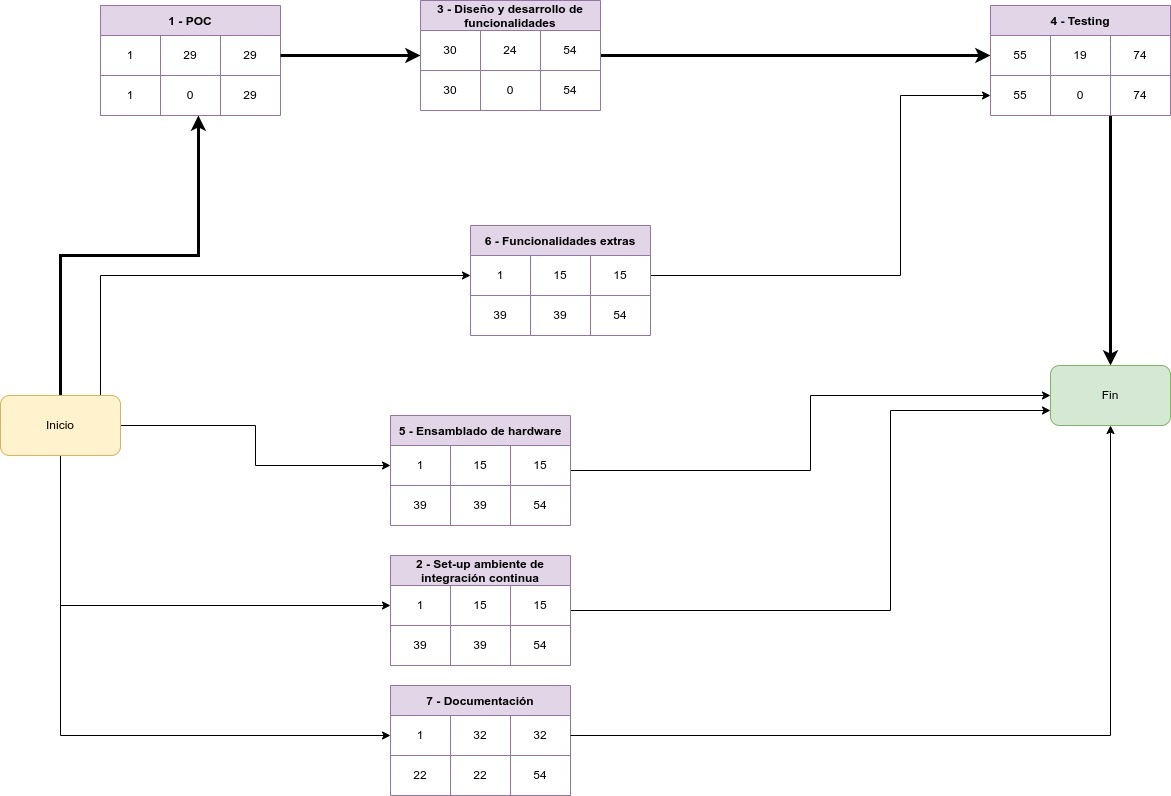
\includegraphics[width=.9\textwidth]{./Figuras/ProyectoFinal-Page-8.jpg}
\caption{Diagrama de \textit{Activity on Node}.}
\label{fig:diagBloques}
\end{figure}
\end{consigna}


\section{11. Diagrama de Gantt}
\label{sec:gantt}

\begin{consigna}{black}

En la siguiente figura, se muestra un ejemplo de diagrama de Gantt realizado con el paquete de \textit{GanttProject}. 

\begin{figure}[htpb]
\centering 
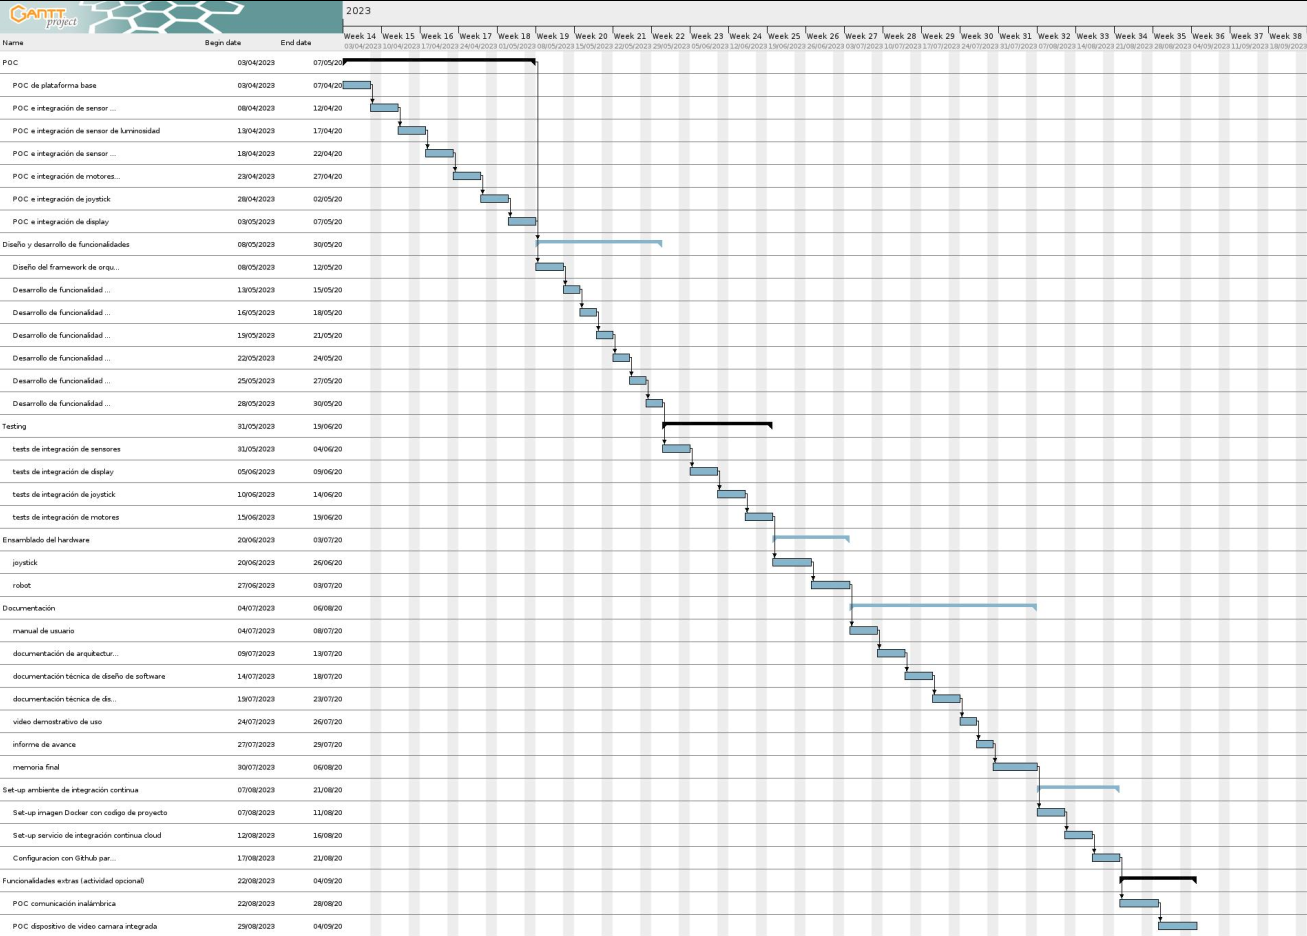
\includegraphics[width=0.95\textwidth]{./Figuras/Captura_Robot_Plan.png}
\caption{Diagrama de Gantt del proyecto}
\label{fig:diagGantt}
\end{figure}
\end{consigna}

\section{12. Presupuesto detallado del proyecto}
\label{sec:presupuesto}

\begin{consigna}{black}

El siguiente cuadro presenta los costos estimados para el proyecto:

\end{consigna}

\begin{table}[htpb]
\centering
\begin{tabularx}{\linewidth}{@{}|X|c|r|r|@{}}
\hline
\rowcolor[HTML]{C0C0C0} 
\multicolumn{4}{|c|}{\cellcolor[HTML]{C0C0C0}COSTOS DIRECTOS} \\ \hline
\rowcolor[HTML]{C0C0C0} 
Descripción &
  \multicolumn{1}{c|}{\cellcolor[HTML]{C0C0C0}Cantidad} &
  \multicolumn{1}{c|}{\cellcolor[HTML]{C0C0C0}Valor unitario} &
  \multicolumn{1}{c|}{\cellcolor[HTML]{C0C0C0}Valor total} \\ \hline
 ESP32 & 
  \multicolumn{1}{c|}{1} &
  \multicolumn{1}{c|}{5000} &
  \multicolumn{1}{c|}{5000} \\ \hline
 Joystick analogico &
  \multicolumn{1}{c|}{1} &
  \multicolumn{1}{c|}{415} &
  \multicolumn{1}{c|}{415} \\ \hline
 Rueditas &
  \multicolumn{1}{c|}{4} &
  \multicolumn{1}{c|}{480} &
  \multicolumn{1}{c|}{1920} \\ \hline
 Sensor BMP280 &
  \multicolumn{1}{c|}{1} &
  \multicolumn{1}{c|}{1255} &
  \multicolumn{1}{c|}{1255} \\ \hline
 Sensor DHT22 &
  \multicolumn{1}{c|}{1} &
  \multicolumn{1}{c|}{2300} &
  \multicolumn{1}{c|}{2300} \\ \hline
 Fotoresitor &
  \multicolumn{1}{c|}{1} &
  \multicolumn{1}{c|}{1220} &
  \multicolumn{1}{c|}{1220} \\ \hline
 Motores DC 3-6 V &
  \multicolumn{1}{c|}{4} &
  \multicolumn{1}{c|}{990} &
  \multicolumn{1}{c|}{3960} \\ \hline
 Cables dupont macho-macho &
  \multicolumn{1}{c|}{1} &
  \multicolumn{1}{c|}{960} &
  \multicolumn{1}{c|}{960} \\ \hline
 Cables dupont macho-hembra &
  \multicolumn{1}{c|}{1} &
  \multicolumn{1}{c|}{960} &
  \multicolumn{1}{c|}{960} \\ \hline
 Plaqueta de cobre para montar &
  \multicolumn{1}{c|}{1} &
  \multicolumn{1}{c|}{1250} &
  \multicolumn{1}{c|}{1250} \\ \hline

\multicolumn{3}{|c|}{SUBTOTAL} &
  \multicolumn{1}{c|}{19240} \\ \hline
\rowcolor[HTML]{C0C0C0} 
\multicolumn{4}{|c|}{\cellcolor[HTML]{C0C0C0}COSTOS INDIRECTOS} \\ \hline
\rowcolor[HTML]{C0C0C0} 
Descripción &
  \multicolumn{1}{c|}{\cellcolor[HTML]{C0C0C0}Cantidad} &
  \multicolumn{1}{c|}{\cellcolor[HTML]{C0C0C0}Valor unitario} &
  \multicolumn{1}{c|}{\cellcolor[HTML]{C0C0C0}Valor total} \\ \hline
\multicolumn{1}{|l|}{-} &
  - &
  - &
  -\\ \hline
\multicolumn{1}{|l|}{-} &
  - &
  - &
  - \\ \hline
\multicolumn{1}{|l|}{-} &
  - &
  - &
  - \\ \hline
\multicolumn{3}{|c|}{SUBTOTAL} &
  \multicolumn{1}{c|}{-} \\ \hline
\rowcolor[HTML]{C0C0C0}
\multicolumn{3}{|c|}{TOTAL} & 19240
   \\ \hline
\end{tabularx}%
\end{table}


\section{13. Gestión de riesgos}
\label{sec:riesgos}

\begin{consigna}{red}
a) Identificación de los riesgos (al menos cinco) y estimación de sus consecuencias:
 
Riesgo 1: detallar el riesgo (riesgo es algo que si ocurre altera los planes previstos de forma negativa)
\begin{itemize}
	\item Severidad (S): mientras más severo, más alto es el número (usar números del 1 al 10).\\
	Justificar el motivo por el cual se asigna determinado número de severidad (S).
	\item Probabilidad de ocurrencia (O): mientras más probable, más alto es el número (usar del 1 al 10).\\
	Justificar el motivo por el cual se asigna determinado número de (O). 
\end{itemize}   

Riesgo 2:
\begin{itemize}
	\item Severidad (S): 
	\item Ocurrencia (O):
\end{itemize}

Riesgo 3:
\begin{itemize}
	\item Severidad (S): 
	\item Ocurrencia (O):
\end{itemize}


b) Tabla de gestión de riesgos:      (El RPN se calcula como RPN=SxO)

\begin{table}[htpb]
\centering
\begin{tabularx}{\linewidth}{@{}|X|c|c|c|c|c|c|@{}}
\hline
\rowcolor[HTML]{C0C0C0} 
Riesgo & S & O & RPN & S* & O* & RPN* \\ \hline
       &   &   &     &    &    &      \\ \hline
       &   &   &     &    &    &      \\ \hline
       &   &   &     &    &    &      \\ \hline
       &   &   &     &    &    &      \\ \hline
       &   &   &     &    &    &      \\ \hline
\end{tabularx}%
\end{table}

Criterio adoptado: 
Se tomarán medidas de mitigación en los riesgos cuyos números de RPN sean mayores a...

Nota: los valores marcados con (*) en la tabla corresponden luego de haber aplicado la mitigación.

c) Plan de mitigación de los riesgos que originalmente excedían el RPN máximo establecido:
 
Riesgo 1: plan de mitigación (si por el RPN fuera necesario elaborar un plan de mitigación).
  Nueva asignación de S y O, con su respectiva justificación:
  - Severidad (S): mientras más severo, más alto es el número (usar números del 1 al 10).
          Justificar el motivo por el cual se asigna determinado número de severidad (S).
  - Probabilidad de ocurrencia (O): mientras más probable, más alto es el número (usar del 1 al 10).
          Justificar el motivo por el cual se asigna determinado número de (O).

Riesgo 2: plan de mitigación (si por el RPN fuera necesario elaborar un plan de mitigación).
 
Riesgo 3: plan de mitigación (si por el RPN fuera necesario elaborar un plan de mitigación).

\end{consigna}


\section{14. Gestión de la calidad}
\label{sec:calidad}

\begin{consigna}{red}
Para cada uno de los requerimientos del proyecto indique:
\begin{itemize} 
\item Req \#1: copiar acá el requerimiento.

\begin{itemize}
	\item Verificación para confirmar si se cumplió con lo requerido antes de mostrar el sistema al cliente. Detallar 
	\item Validación con el cliente para confirmar que está de acuerdo en que se cumplió con lo requerido. Detallar  
\end{itemize}

\end{itemize}

Tener en cuenta que en este contexto se pueden mencionar simulaciones, cálculos, revisión de hojas de datos, consulta con expertos, mediciones, etc.  Las acciones de verificación suelen considerar al entregable como ``caja blanca'', es decir se conoce en profundidad su funcionamiento interno.  En cambio, las acciones de validación suelen considerar al entregable como ``caja negra'', es decir, que no se conocen los detalles de su funcionamiento interno.

\end{consigna}

\section{15. Procesos de cierre}    
\label{sec:cierre}

\begin{consigna}{red}
Establecer las pautas de trabajo para realizar una reunión final de evaluación del proyecto, tal que contemple las siguientes actividades:

\begin{itemize}
	\item Pautas de trabajo que se seguirán para analizar si se respetó el Plan de Proyecto original:
	 - Indicar quién se ocupará de hacer esto y cuál será el procedimiento a aplicar. 
	\item Identificación de las técnicas y procedimientos útiles e inútiles que se emplearon, y los problemas que surgieron y cómo se solucionaron:
	 - Indicar quién se ocupará de hacer esto y cuál será el procedimiento para dejar registro.
	\item Indicar quién organizará el acto de agradecimiento a todos los interesados, y en especial al equipo de trabajo y colaboradores:
	  - Indicar esto y quién financiará los gastos correspondientes.
\end{itemize}

\end{consigna}


\end{document}
